\newpage
\section{Realisering}
\label{realiseringOgTest}

\subsection{Kretstopologi og bestemmelse av variabelverdier}

Beregna variabelverdier til det endelige systemet vises i tabell \ref{tab:vars}.

\vspace{1cm}
\begin{table}[!h]
\centering % Denne kommandoen sentrerer tabellen i kolonnen. 
\caption{Beregna verdier.}
\label{tab:vars}	% Merkelappen vi vil referere til.
\begin{tabular}{lll} % Her angir det andre argumentet at vi vil ha to senterjusterte kolonner (l = left, c = center, r = right).
\toprule % Horisontal linje som markerer toppen av tabellen
\textbf{Variabel/komponent} & \textbf{Beregna verdi} \\
\midrule
$f_\text{s}$ & $3.4\text{ kHz}$ \\
$f_B$ & $1.7\text{ kHz}$ \\
$f_c$ & $1.275\text{ kHz}$ \\
$n$ & $4$ \\
\bottomrule 
\end{tabular}
\end{table}
\vspace{1cm}

Ettersom vi kommer til å fastsette kondensatorene og beregne motstandene så setter vi opp et sjette ordens system. Vi benytter oss da av 3 SallenKey-koblinger i kaskade med verdier som gitt i tabell \ref{tab:verdier}.

\begin{table}[!h]
    \centering
    \caption{Verdier for Sallen-Key-koblingene.}
    \label{tab:verdier}
    \begin{tabular}{lllll}
    Sallen Key & R1  & C1  & R2  & C2  \\
    1          & $220\Omega$ & $2.5\mu$F & $220\Omega$ & $100$nF \\
    2          & $680\Omega$ & $330$nF & $680\Omega$ & $100$nF \\
    3          & $100\Omega$ & $1.5\mu$F & $100\Omega$ & $1\mu$F  
    \end{tabular}
    \end{table}

Den oppkoblete kretsen kan sees i figur \ref{fig:oppkobling}.

\begin{figure}[!h]
    \centering
    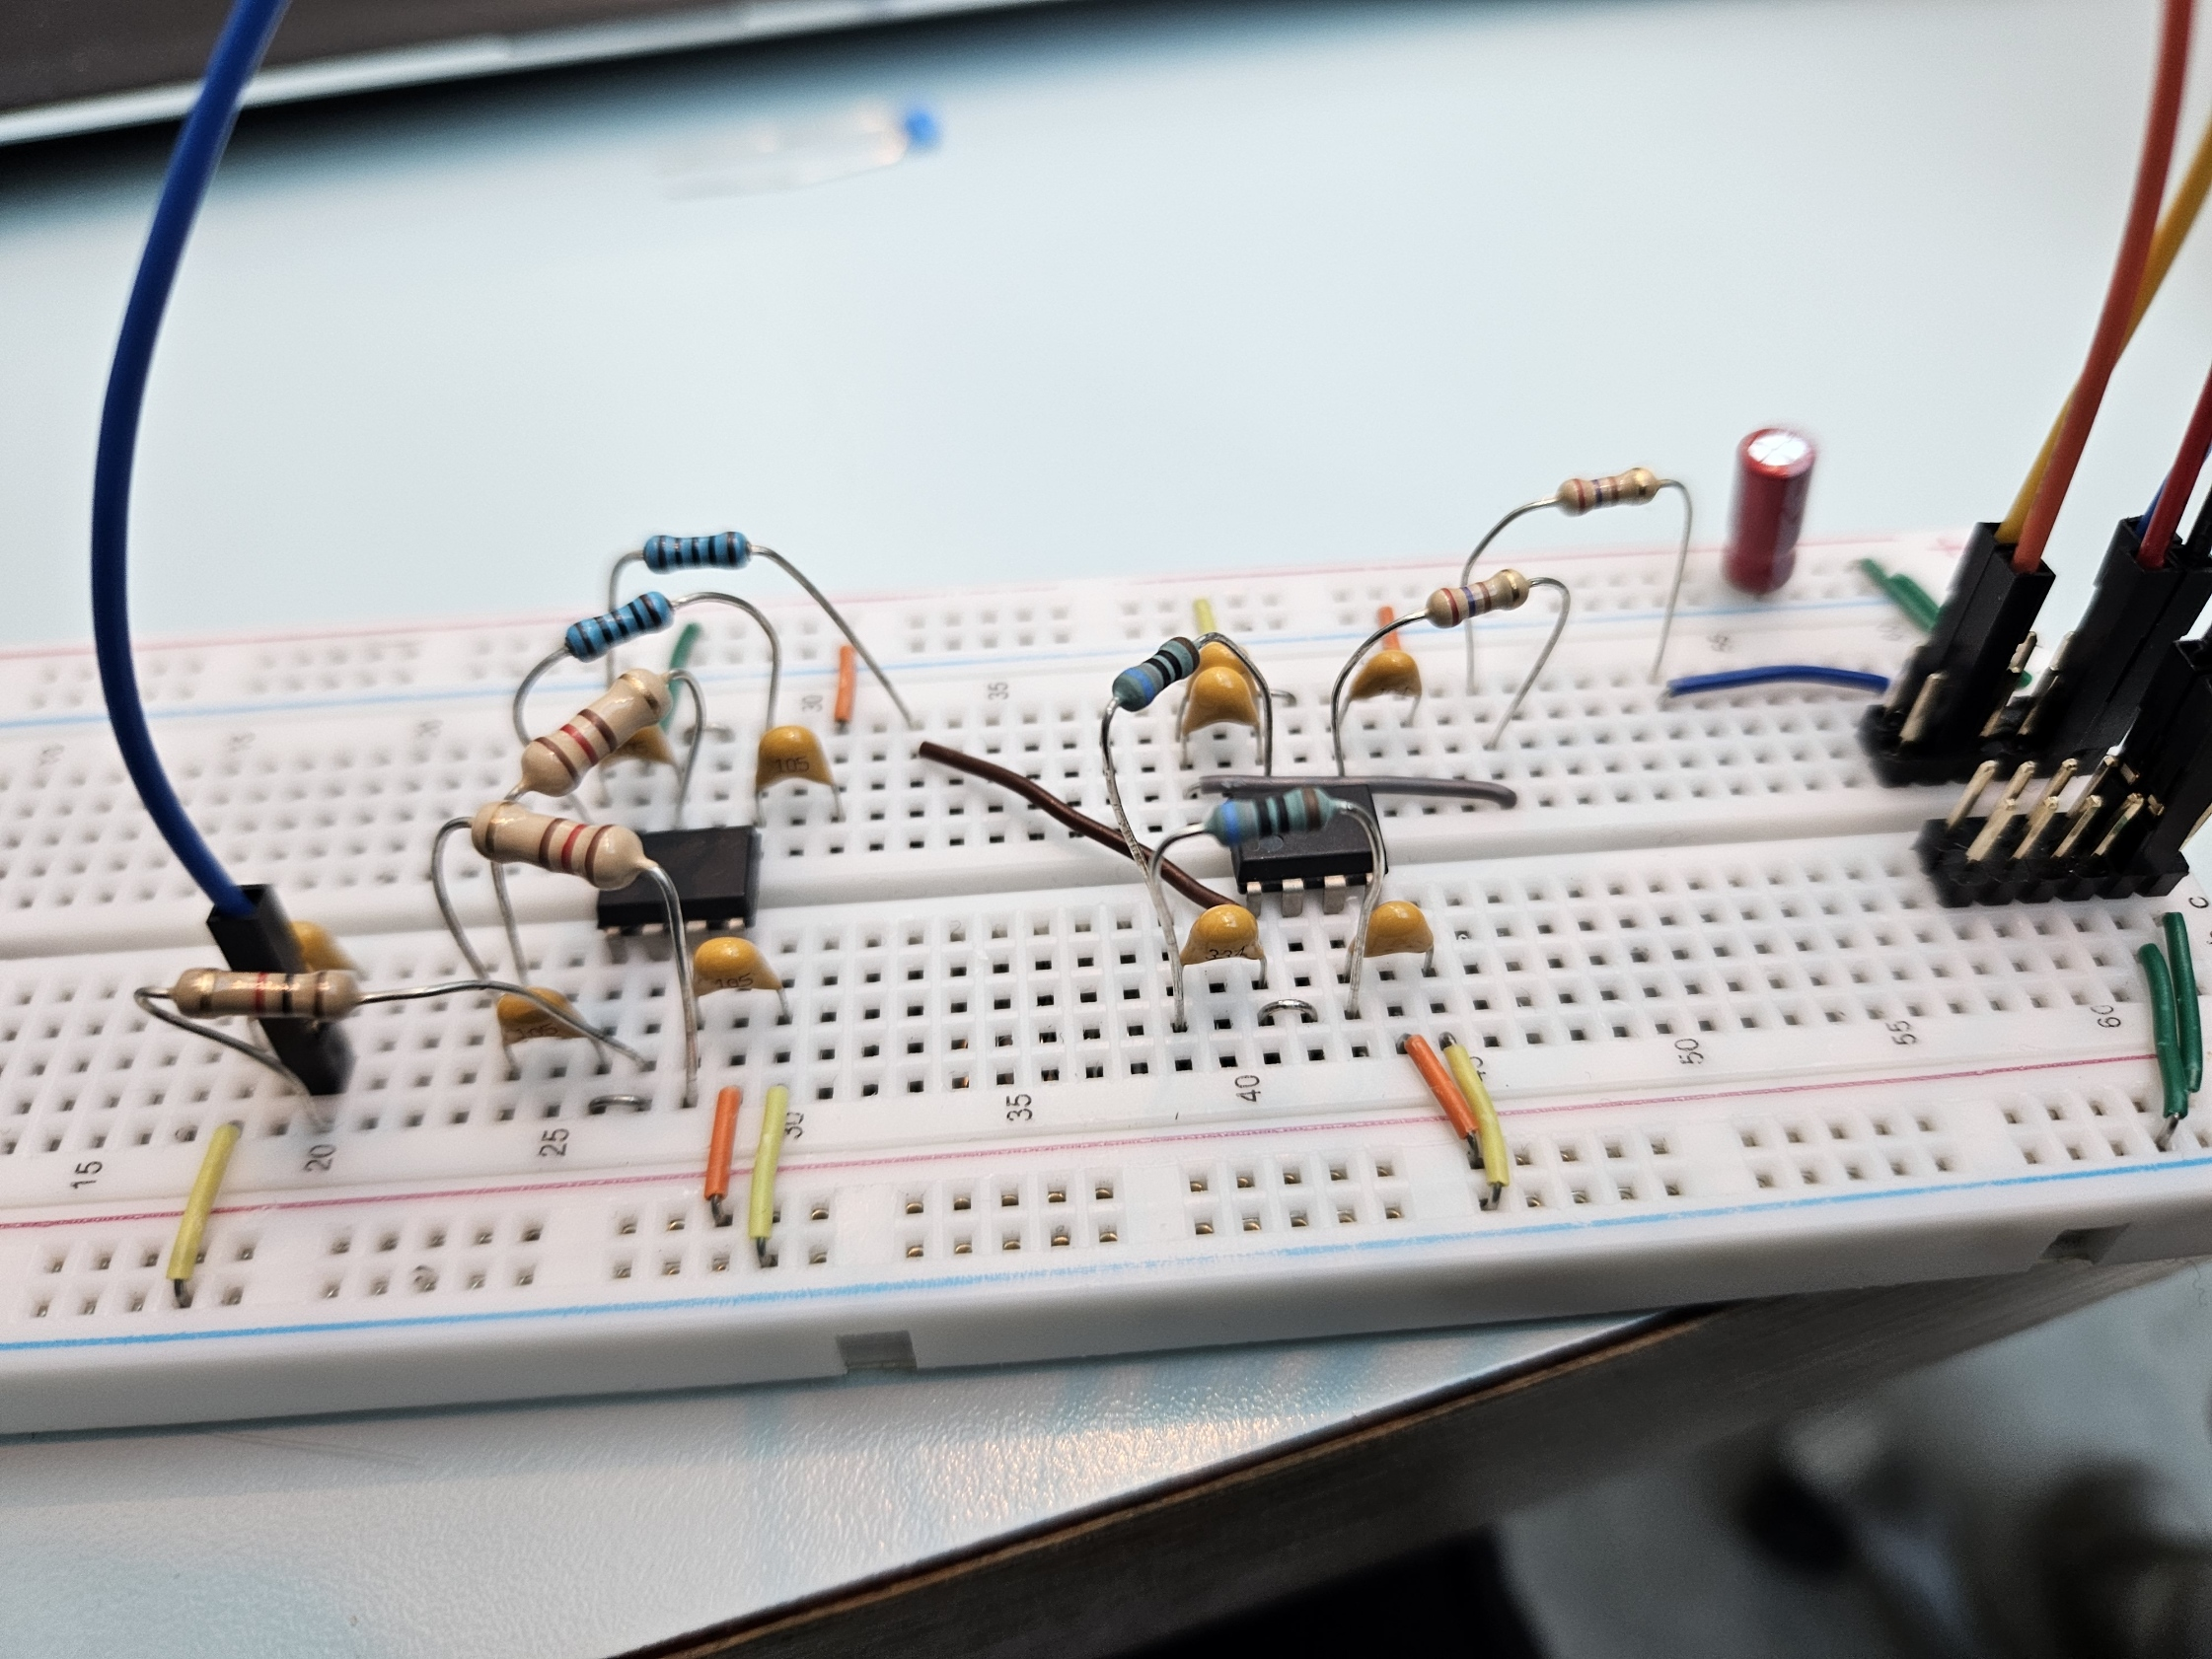
\includegraphics[width=0.8\textwidth]{Bilder/OppkoblingButterworth.jpg}
    \caption{Oppkobling av kretsen.}
    \label{fig:oppkobling}
\end{figure}
\newpage
\subsection{Resultater}
Etter at kretsen var koblet opp ble det målt på amplituderesponsen til filteret. Dette ble gjort ved å sende inn et signal med frekvenser fra $0$ til $100\text{ kHz}$ ved hjelp av en netverksanalysator. Resultatet av målingene kan sees i figur \ref{fig:amplituderespons}.



\begin{figure}[!h]
    \centering
    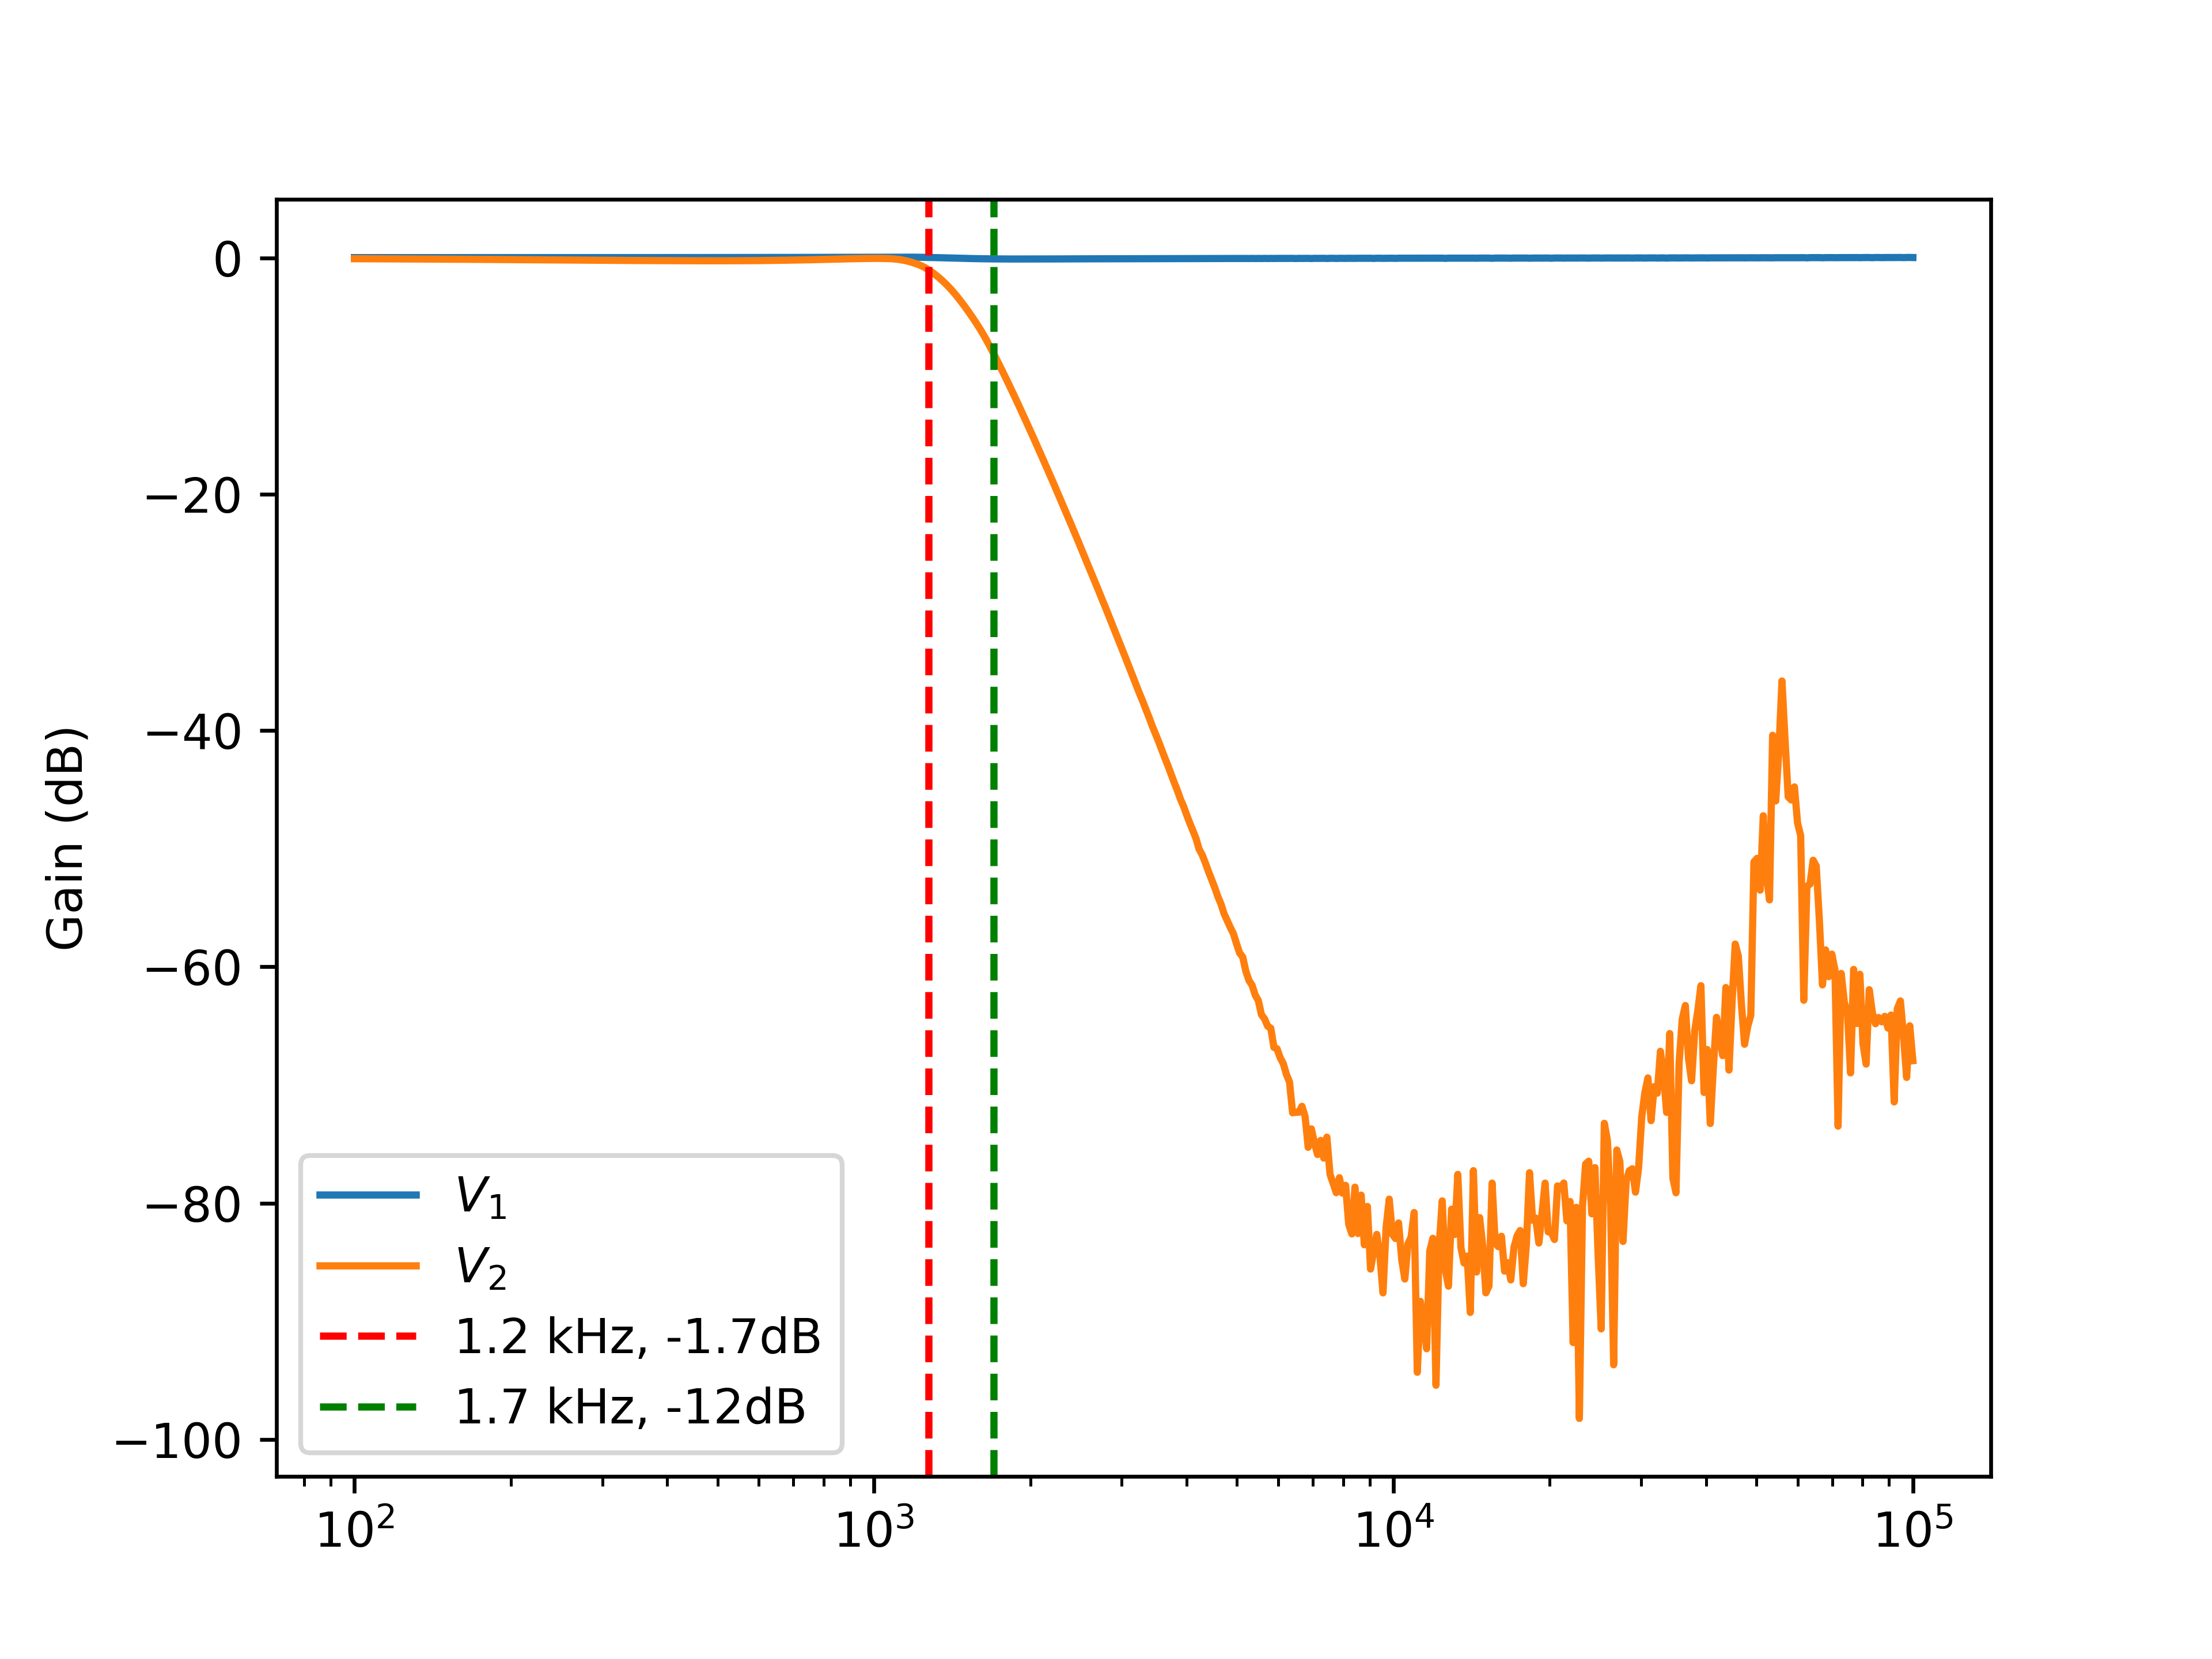
\includegraphics[width=0.8\textwidth]{Bilder/bode.png}
    \caption{Amplituderesponsen til filteret.}
    \label{fig:amplituderespons}    
\end{figure}

\newpage